%%%%%%%%%%%%%%%%%%%%%%%%%%%%%%%%%%%%%%%%%%%%%%%%%%%%%%%%%%%%%%%%%%%%%%%%%%%%%%%%
%2345678901234567890123456789012345678901234567890123456789012345678901234567890
%        1         2         3         4         5         6         7         8

\documentclass[letterpaper, 10 pt, conference]{ieeeconf}  % Comment this line out if you need a4paper
\usepackage{cite}
\usepackage{amsmath,amssymb,amsfonts}
\usepackage{algorithmic}
\usepackage{graphicx}
\usepackage{textcomp}
\usepackage{xcolor}

%\documentclass[a4paper, 10pt, conference]{ieeeconf}      % Use this line for a4 paper

\IEEEoverridecommandlockouts                              % This command is only needed if 
                                                          % you want to use the \thanks command

\overrideIEEEmargins                                      % Needed to meet printer requirements.

%In case you encounter the following error:
%Error 1010 The PDF file may be corrupt (unable to open PDF file) OR
%Error 1000 An error occurred while parsing a contents stream. Unable to analyze the PDF file.
%This is a known problem with pdfLaTeX conversion filter. The file cannot be opened with acrobat reader
%Please use one of the alternatives below to circumvent this error by uncommenting one or the other
%\pdfobjcompresslevel=0
%\pdfminorversion=4

% See the \addtolength command later in the file to balance the column lengths
% on the last page of the document

% The following packages can be found on http:\\www.ctan.org
%\usepackage{graphics} % for pdf, bitmapped graphics files
%\usepackage{epsfig} % for postscript graphics files
%\usepackage{mathptmx} % assumes new font selection scheme installed
%\usepackage{times} % assumes new font selection scheme installed
%\usepackage{amsmath} % assumes amsmath package installed
%\usepackage{amssymb}  % assumes amsmath package installed

\title{\LARGE \bf
Homework 3 - Option 1\\
\small{UCLA MAE 263F, Fall 2024\\
Mechanics of Flexible Structures and Soft Robots}%
}


\author{He Kai Lim$^{1}$ % <-this % stops a space
\thanks{$^{1}$He Kai Lim is with the 
Department of Mechanical and Aerospace Engineering, 
University of California Los Angeles, Los Angeles, CA 90095 USA
        {\tt\small limhekai@ucla.edu}}%
}


\begin{document}

\maketitle
\thispagestyle{empty}
\pagestyle{empty}


%%%%%%%%%%%%%%%%%%%%%%%%%%%%%%%%%%%%%%%%%%%%%%%%%%%%%%%%%%%%%%%%%%%%%%%%%%%%%%%%
\begin{abstract}
   This report strives to provide all deliverables for Homework 3 in partial fulfilment of the requirements for UCLA MAE 263F, Fall 2024 (Mechanics of Flexible Structures and Soft Robots)
\end{abstract}


%%%%%%%%%%%%%%%%%%%%%%%%%%%%%%%%%%%%%%%%%%%%%%%%%%%%%%%%%%%%%%%%%%%%%%%%%%%%%%%%
\section{INTRODUCTION}
Fits are important to perform good science, and machine-learned iterative methods are a useful method to create these linear fits when the data is unintuitive.
There are two main types of fits: linear and nonlinear.
Both need to be carefully examined to understand the methods of implementing machine learning methods in creating these fits.



%%%%%%%%%%%%%%%%%%%%%%%%%%%%%%%%%%%
\section{Problem 1 - Linear Fits}

Here, we want to fit data to a linear equation:
\begin{equation}
   y = mx + b
\end{equation}

\subsection{Theory}

We use the Mean Squared Error (MSE) loss function:

\begin{equation}
   \text{Loss}(m,b) = \frac{1}{N} \sum^{N}_{i=1}(y_i - (m \cdot x_i + b) )^2
\end{equation}

The gradients of the loss function with respect to \textit{m} and \textit{b} are:

\begin{equation}
   \frac{\partial \text{Loss}}{\partial m}
   =
   -\frac{2}{N}\sum^{N}_{i=1}x_i \cdot (y_i - (m \cdot x_i + b) )
\end{equation}

\begin{equation}
   \frac{\partial \text{Loss}}{\partial b}
   =
   -\frac{2}{N}\sum^{N}_{i=1} (y_i - (m \cdot x_i + b) )
\end{equation}

Using gradient descent, we update the hyperparameters \textit{m} and \textit{b} as follows:

\begin{equation}
   m \leftarrow m - \eta \frac{\partial \text{Loss}}{\partial m}, b \leftarrow b - \eta\frac{\partial \text{Loss}}{\partial b}
\end{equation}

where $\eta$ is the learning rate.

\subsection{Results: 1a}
Compare the predicted values with the actual data. 
After fitting the model, plot the predicted values $y_{pred}$ versus the actual data $y$. Include the plot in your report. 

These are the results of fitting the model for 10000 epochs at a learning rate of 0.001.

\begin{table}[h]
   \centering
   \caption{Linear Fit: Nominal values of $m_{fit}$ and $b_{fit}$}
   \label{tab:Lin_Nominal_mb}
   \begin{tabular}{|c|c|}
      \hline
      $m_{fit}$ & $b_{fit}$ \\
      \hline
      -0.011781642379859762 & 0.06320409591699154 \\
      \hline
   \end{tabular}
\end{table}

% [h!] makes latex try to place figure exactly there, not floating around
\begin{figure}[h!]
   \centering
   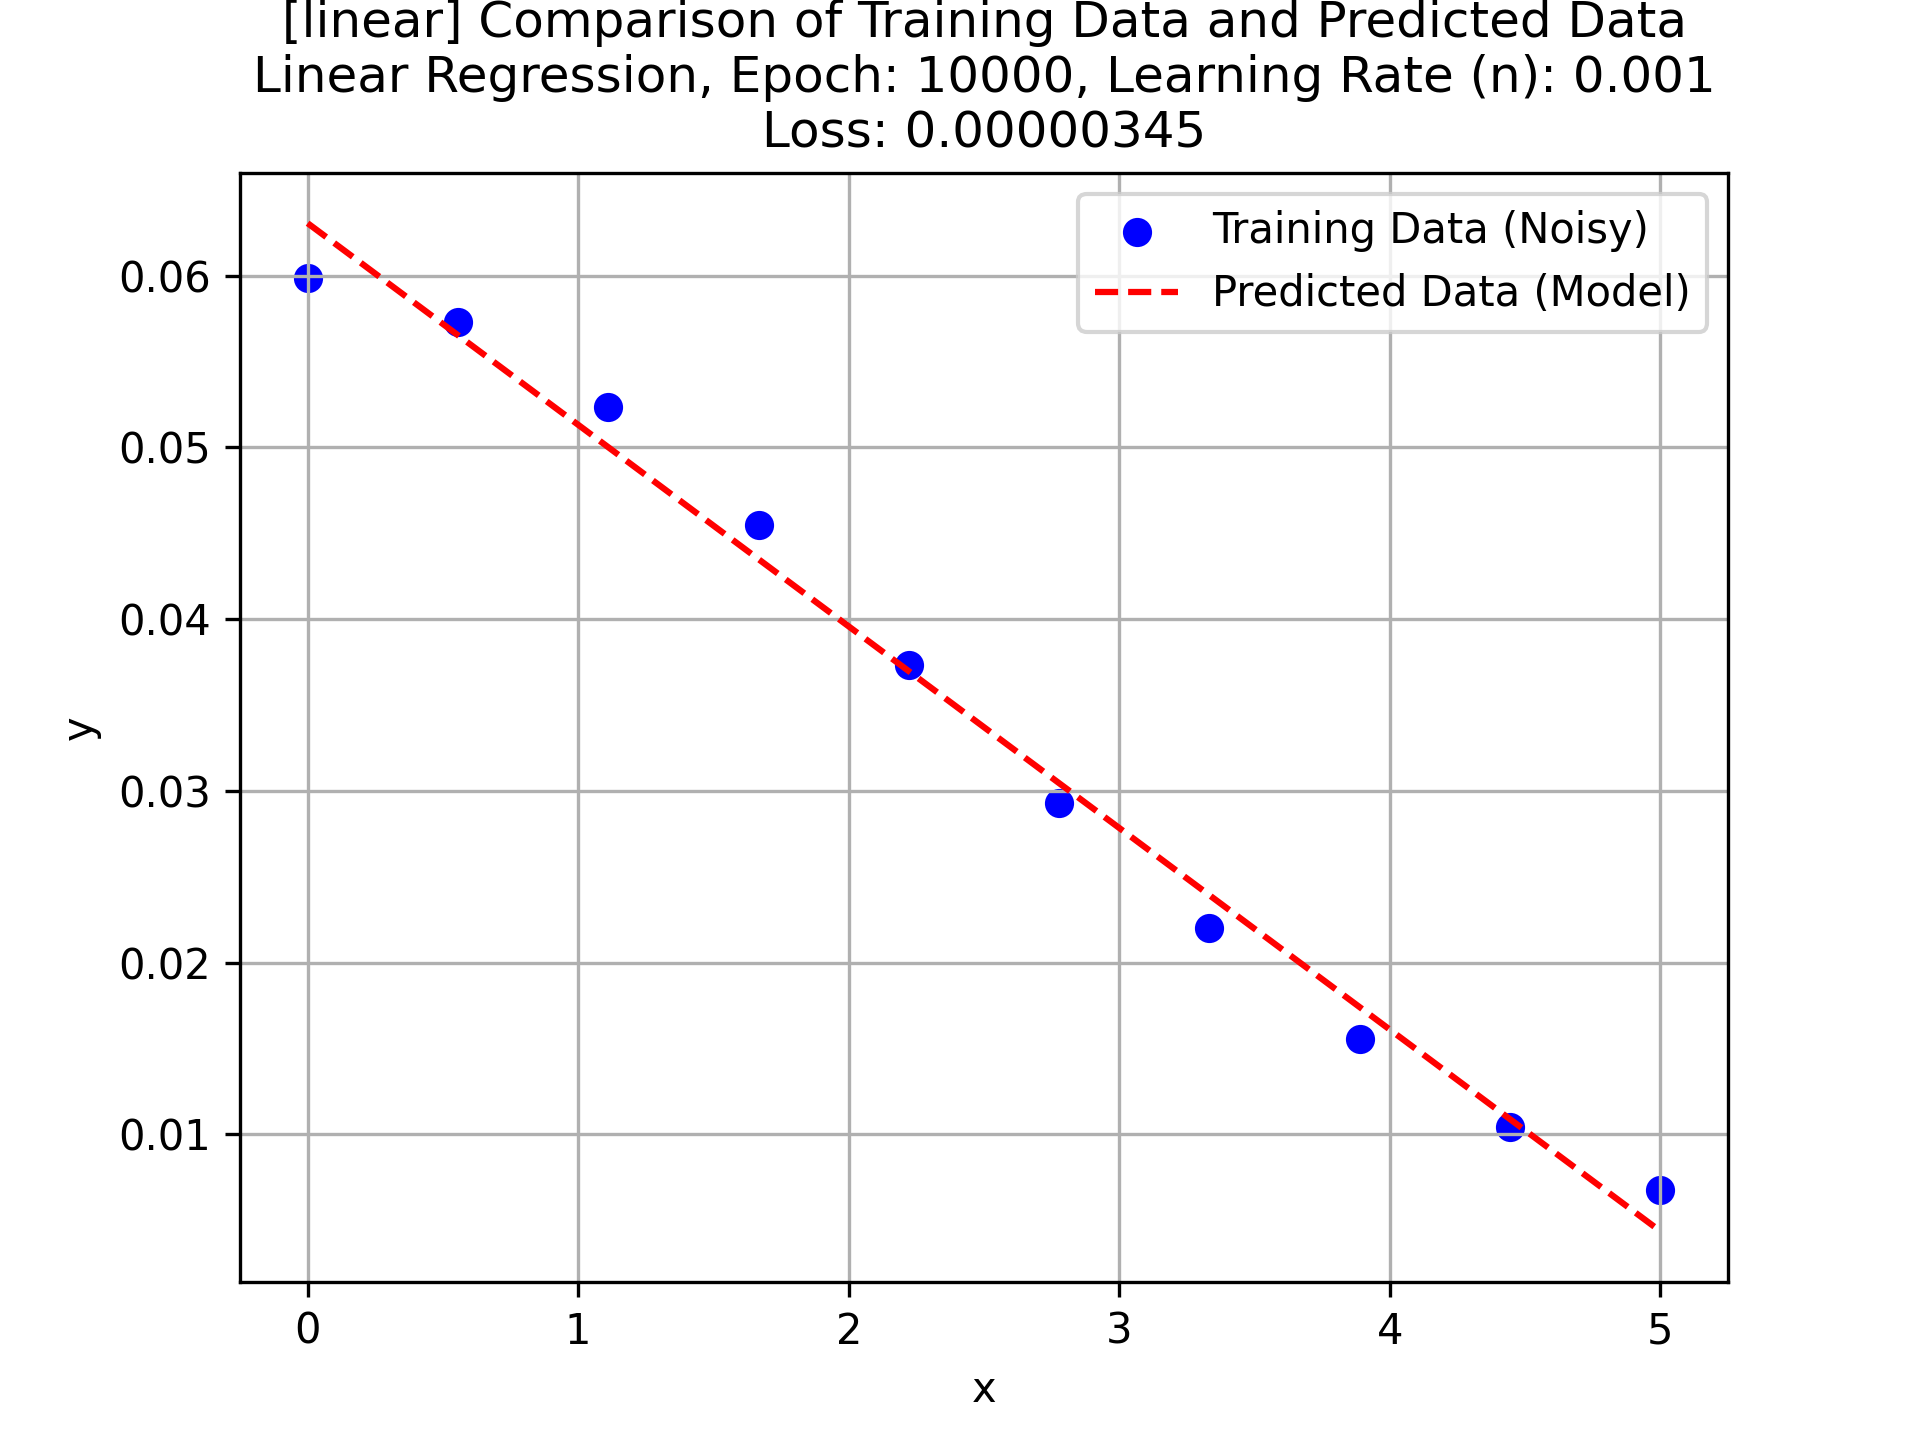
\includegraphics[width=0.8\linewidth]{../Figures/linear_regression_e_10000_n_0.001.png}
   \caption{Predicted values $y_{pred}$ versus actual data $y$ with original values }
   \label{fig:Lin_a}
\end{figure}


\subsection{Results: 1b}
Problem 1b: Experiment with the learning rate and number of epochs.

Here I manually tried different values of epochs and learning rate ($\eta$) and found the set that minimized loss with ensured convergence

\begin{table}[h]
   \centering
   \caption{Linear Fit: Table of hyperparameters}
   \label{tab:lin_param}
   \begin{tabular}{|c|c|c|c|c|}
      \hline
      Epoch & Learning Rate ($\eta$) & Loss & Convergence & Figure\\
      \hline
      10000 & 0.001 & 0.00000391 & Yes & \ref{fig:Lin_a}\\
      \hline
      1000 & 0.001 & 0.02600305 & No\ & \ref{fig:Lin_b_less_e}\\
      \hline
      10000 & 0.01 & 0.00000343 & Yes & \ref{fig:Lin_b_less_n}\\
      \hline
      1000 & 0.01 & 0.00000343 & Yes & \ref{fig:Lin_b_min_loss}\\
      \hline
   \end{tabular}
   
\end{table}


% [h!] makes latex try to place figure exactly there, not floating around
\begin{figure}[h!]
   \centering
   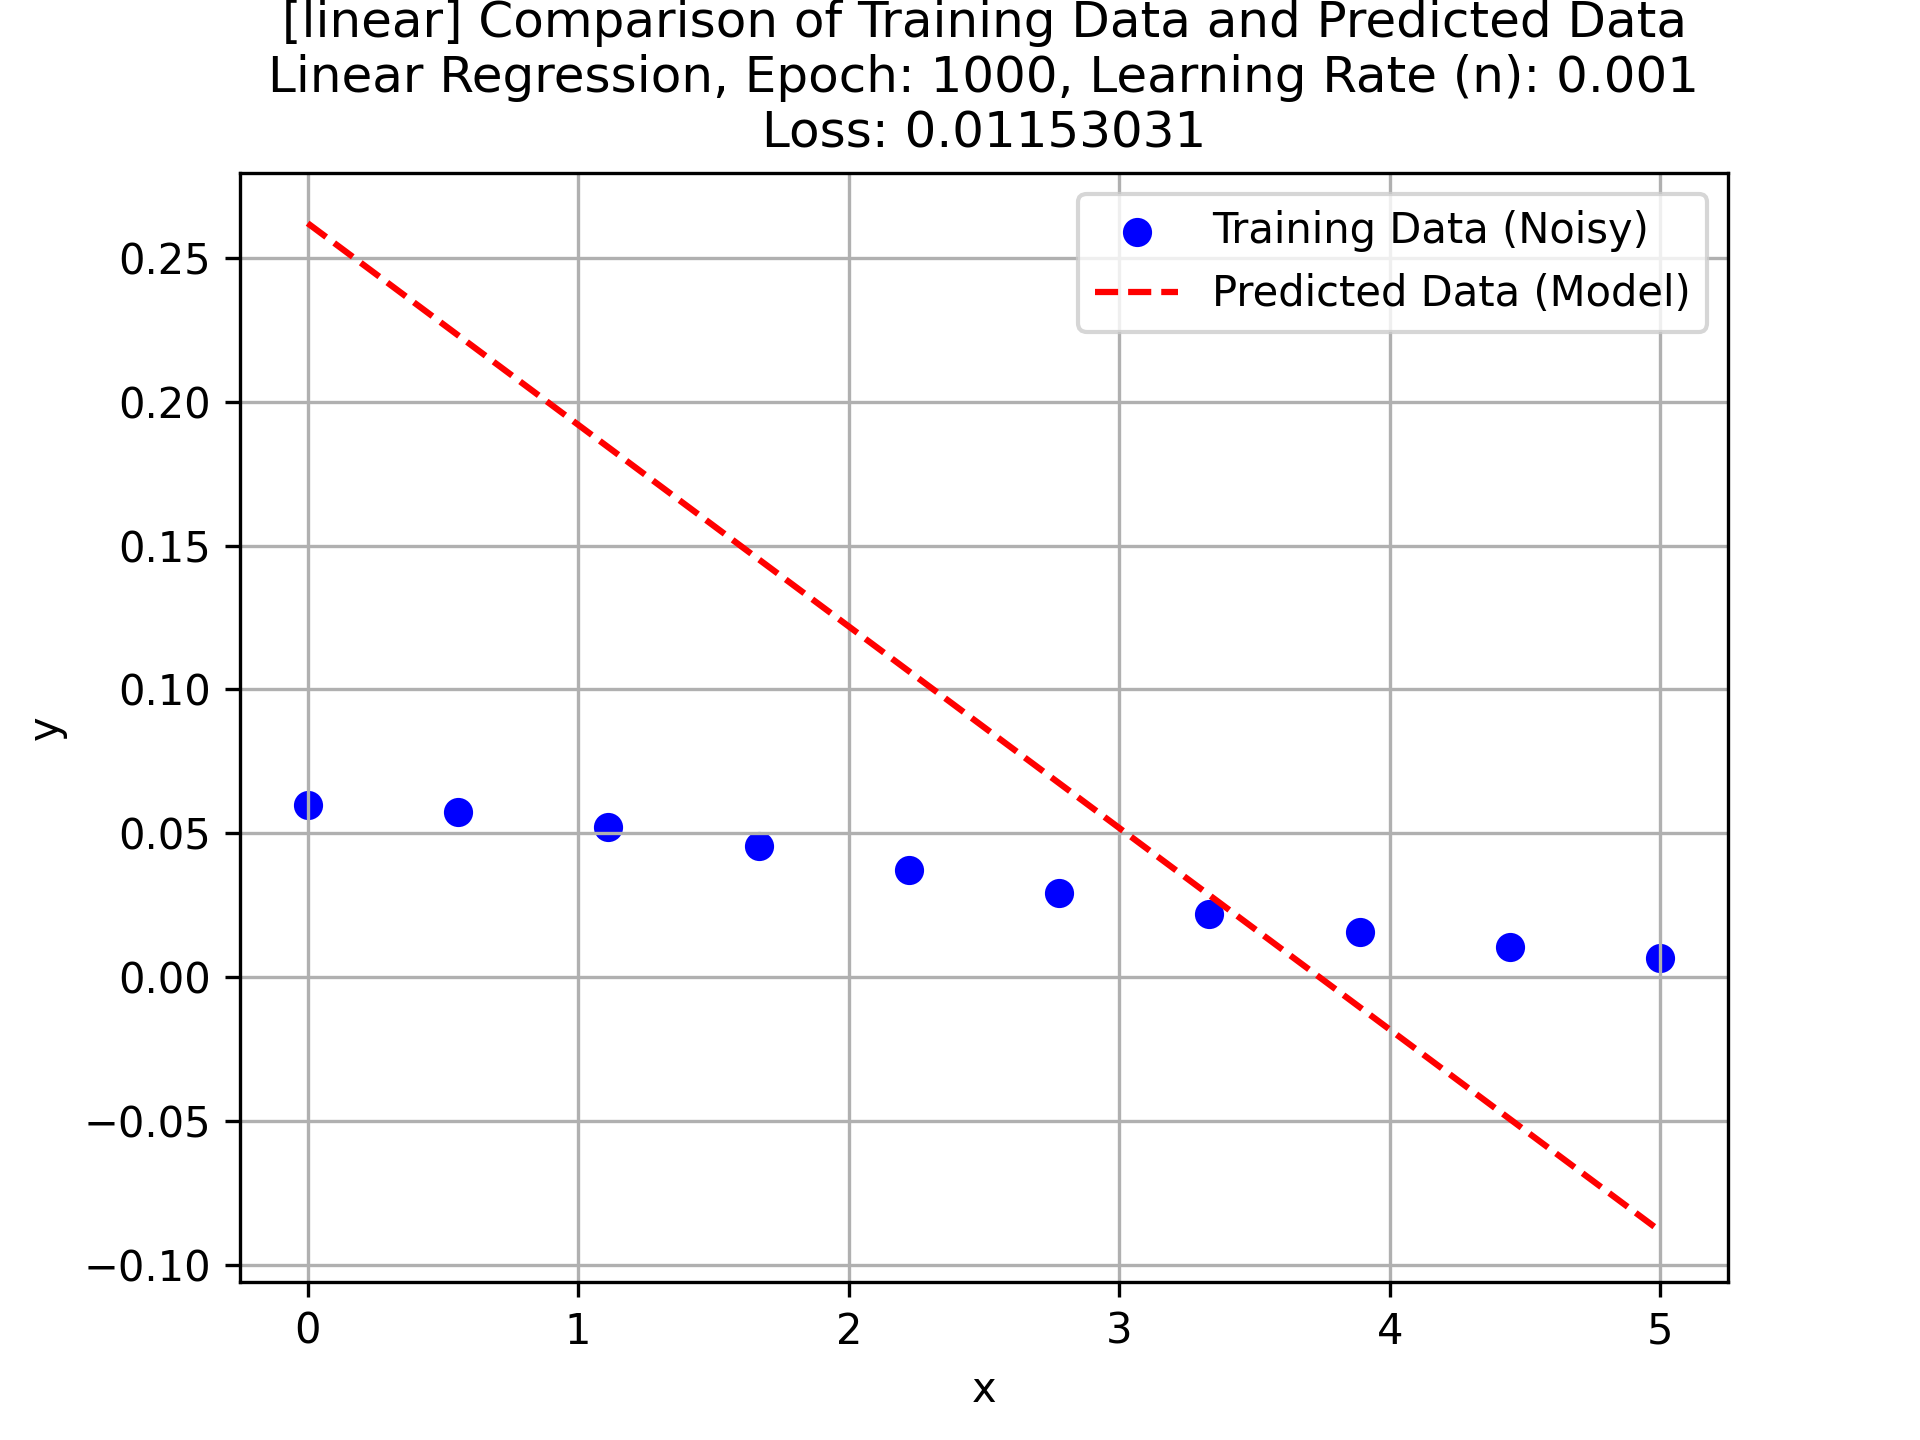
\includegraphics[width=0.8\linewidth]{../Figures/linear_regression_e_1000_n_0.001.png}
   \caption{Predicted values $y_{pred}$ versus actual data $y$ with no convergence}
   \label{fig:Lin_b_less_e}
\end{figure}

% [h!] makes latex try to place figure exactly there, not floating around
\begin{figure}[h!]
   \centering
   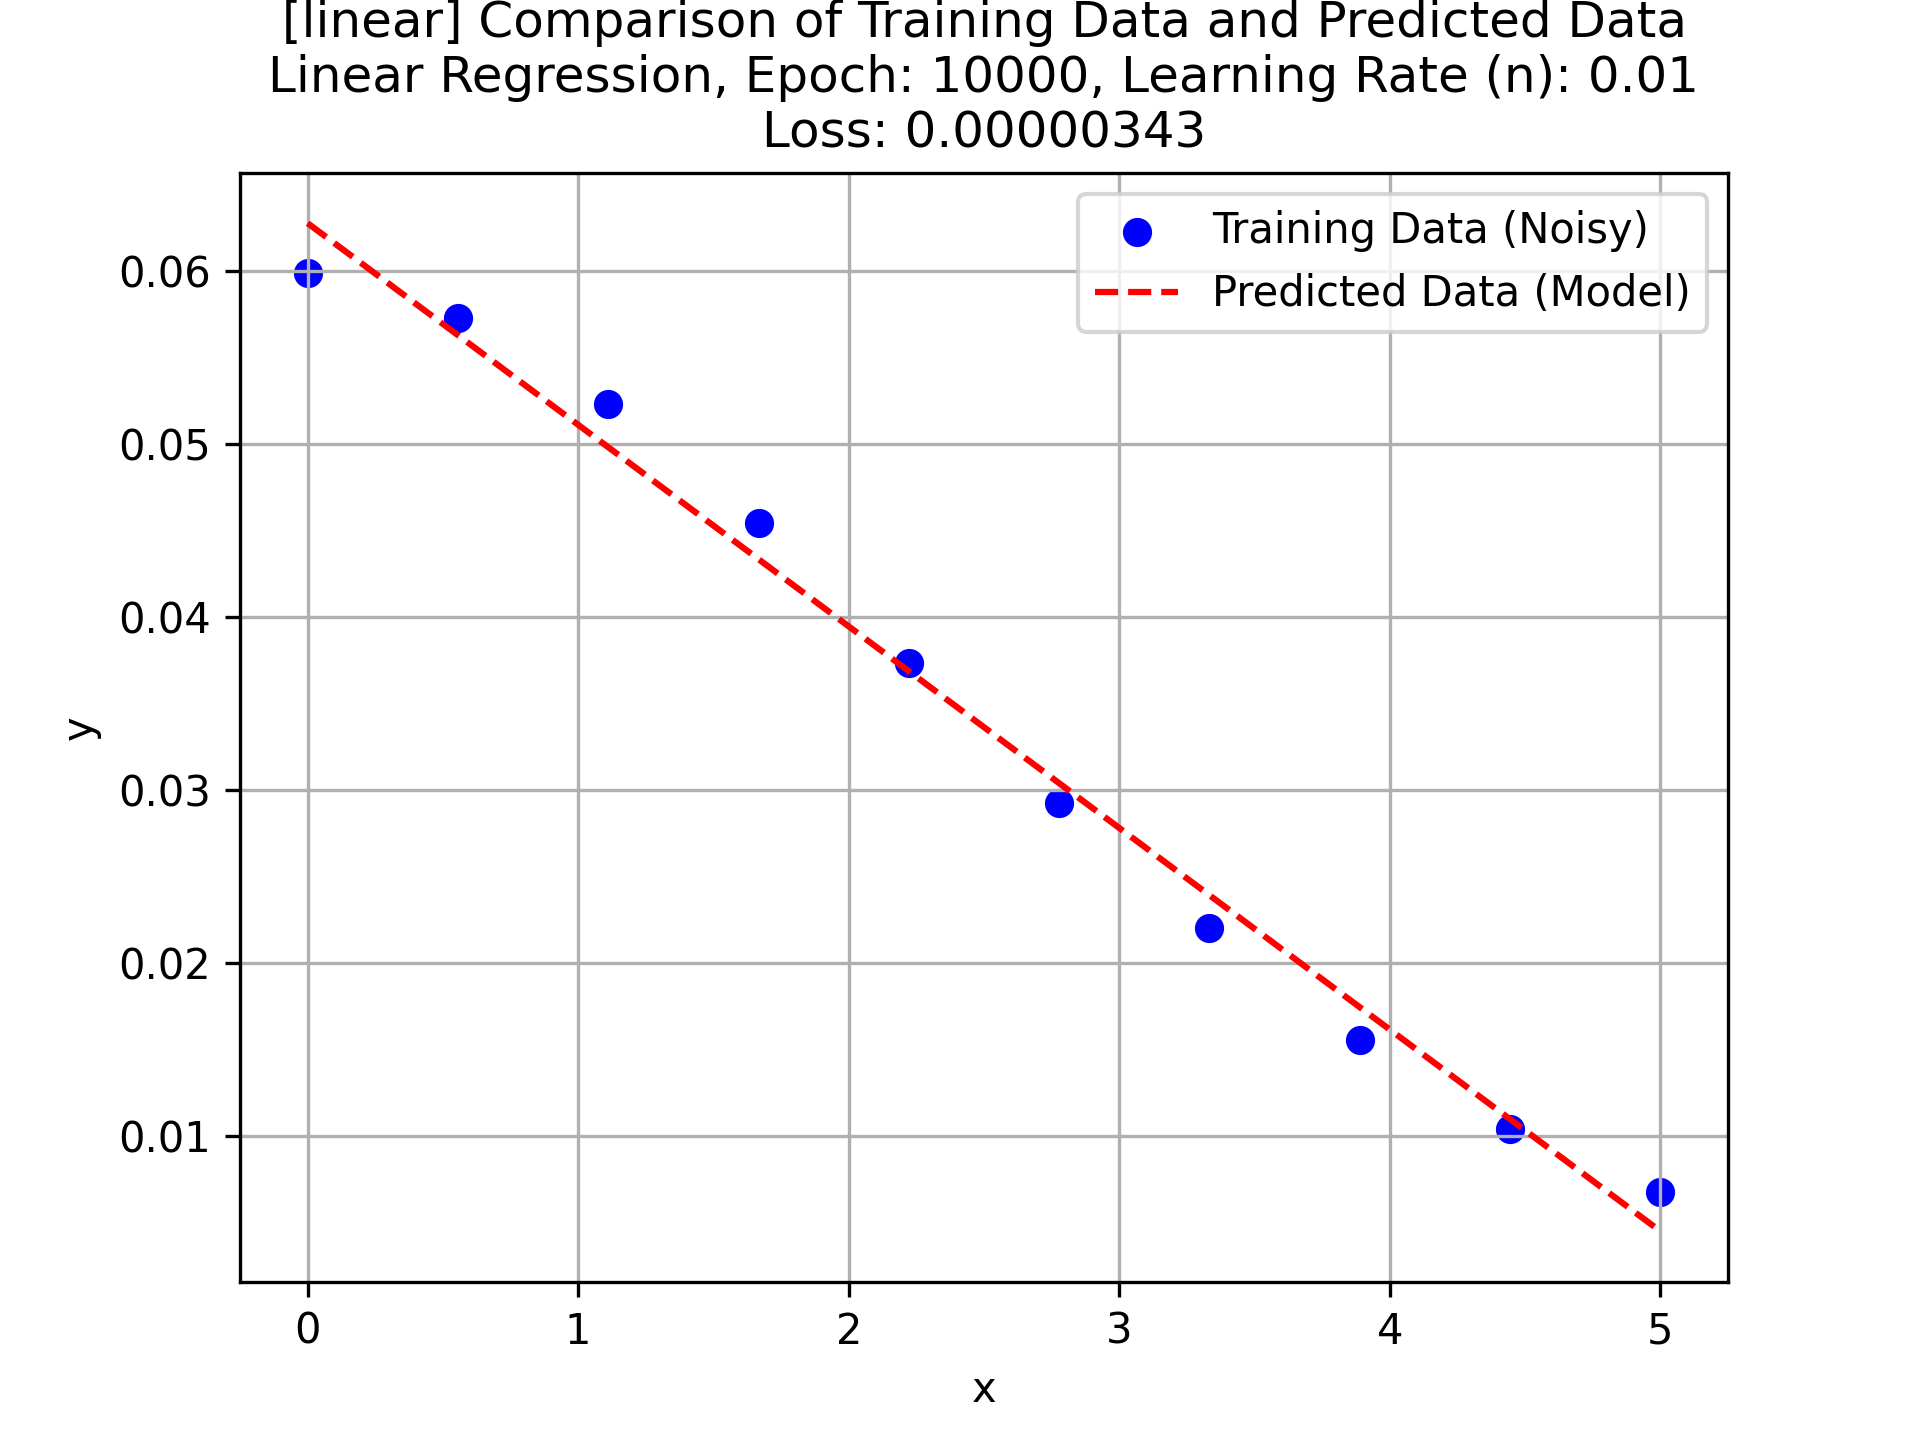
\includegraphics[width=0.8\linewidth]{../Figures/linear_regression_e_10000_n_0.01.png}
   \caption{Predicted values $y_{pred}$ versus actual data $y$ with minimum loss but excess epochs}
   \label{fig:Lin_b_less_n}
\end{figure}

% [h!] makes latex try to place figure exactly there, not floating around
\begin{figure}[h!]
   \centering
   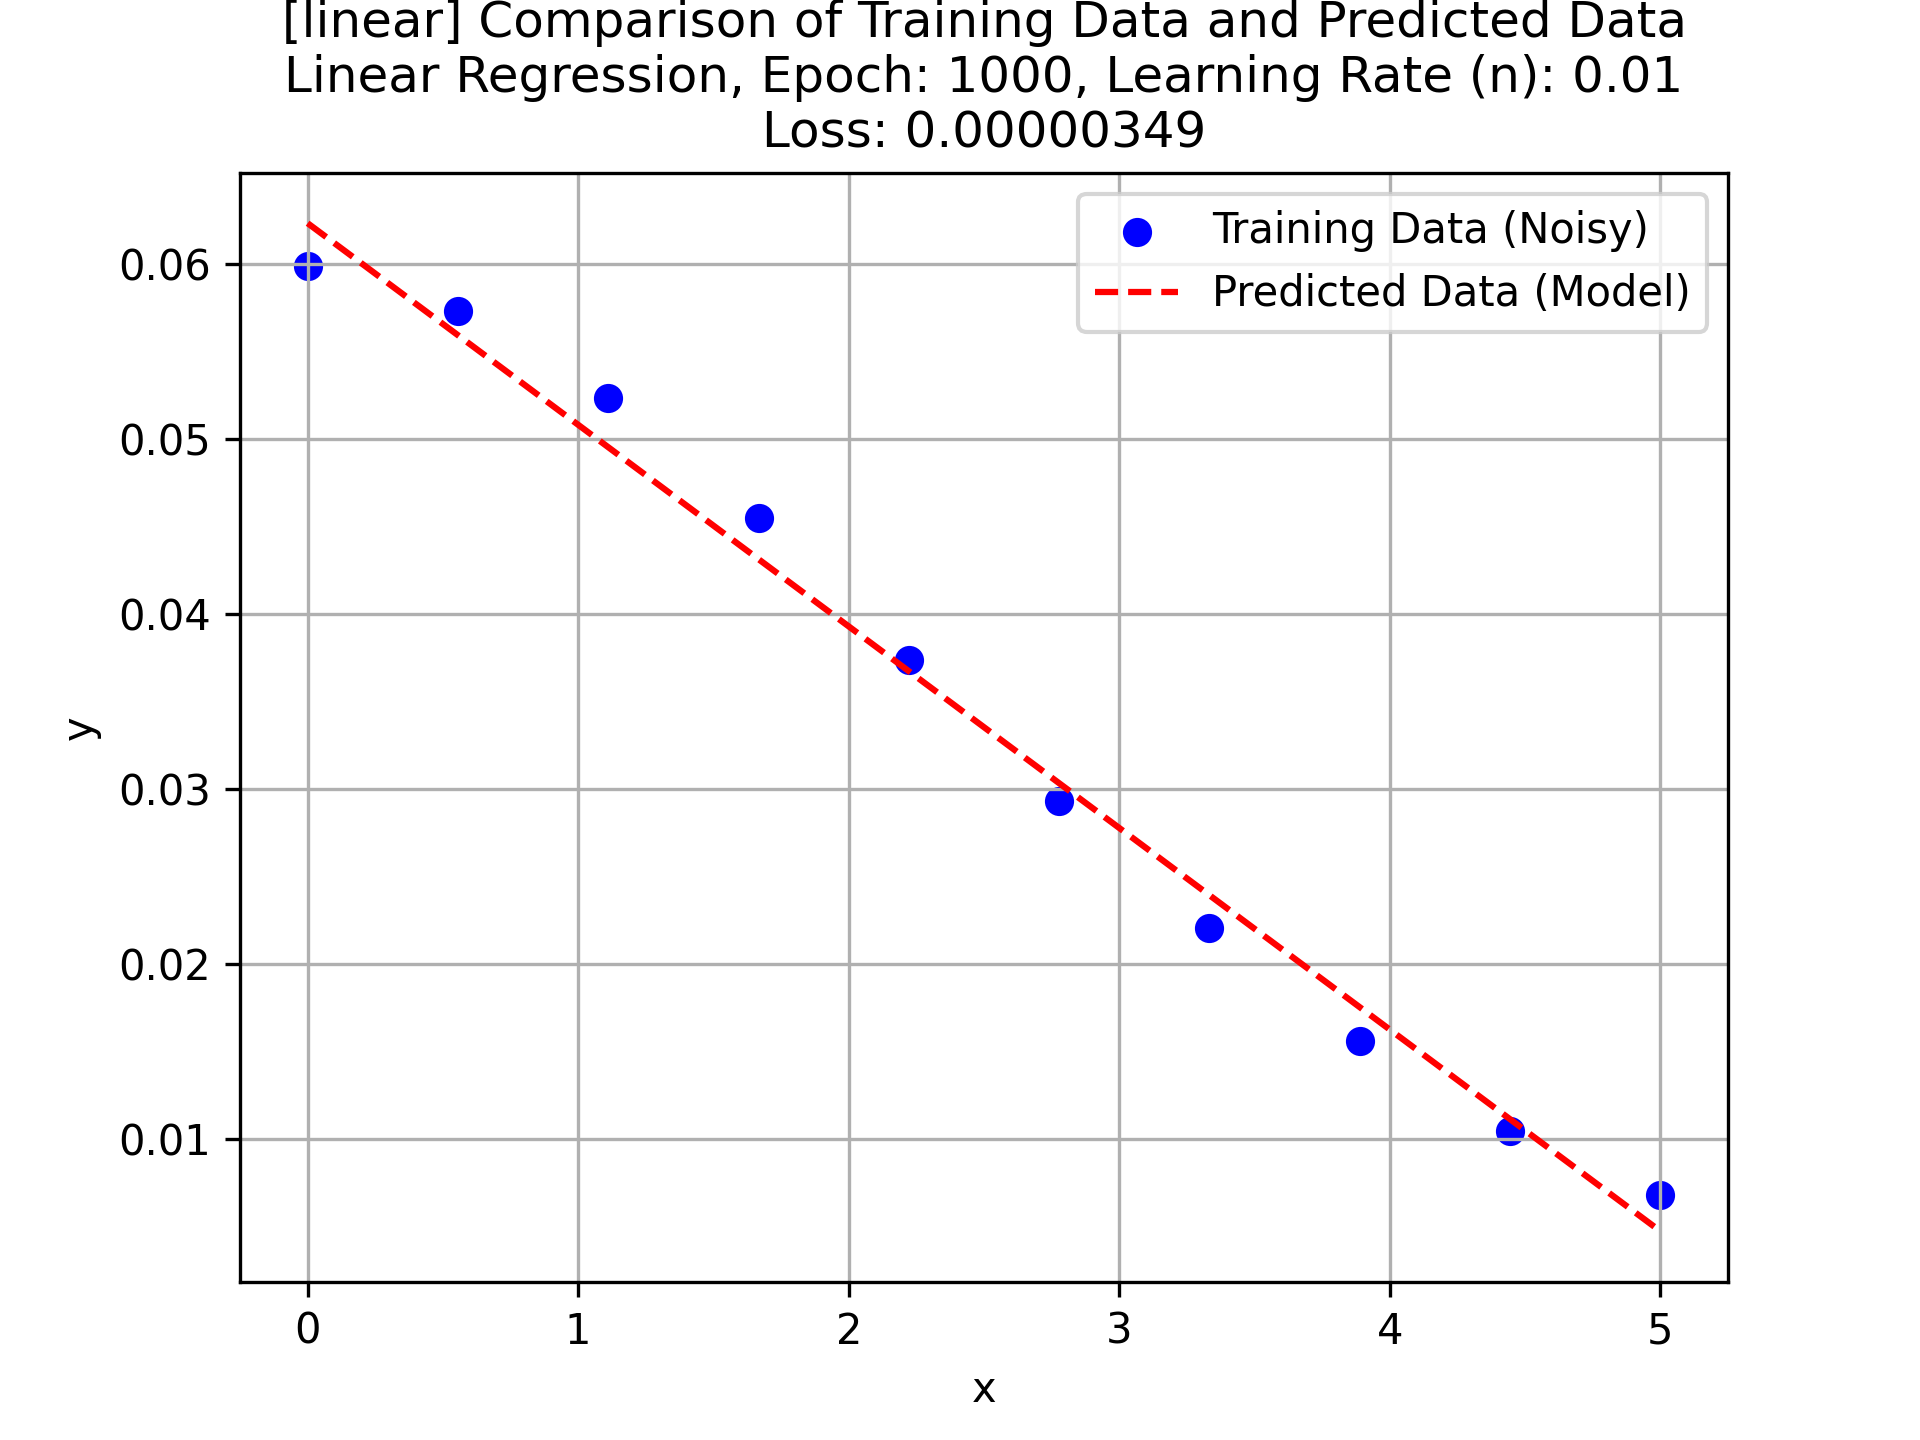
\includegraphics[width=0.8\linewidth]{../Figures/linear_regression_e_1000_n_0.01.png}
   \caption{Predicted values $y_{pred}$ versus actual data $y$ with minimum loss and optimized epochs}
   \label{fig:Lin_b_min_loss}
\end{figure}

Changing the learning rate effects the number of epochs required for convergence. 
A smaller learning rate requires more epochs before convergence.
Furthermore, a larger learning rate also affects the precision of the fit, meaning that a minimum loss might not be found because of the larger "steps" from the learning rate. 

Changing the number of epochs affects the final loss, assuming loss is not yet minimized. 
This means there is a minimum number of epochs required to get the optimum fit, and thereafter, higher numbers of epochs are wasted a computation resource.

Together, this means we want a learning rate that is just large enough to find the minimum loss fit, then we want to minimize the number of epochs within this fit.
This was manually found and presented in Figure. \ref{fig:Lin_b_min_loss}. 

%%%%%%%%%%%%%%%%%%%%%%%%%%%%%%%%%%%
\section{Problem 2 - Nonlinear Fits}

\subsection{Theory}

Here, we want to fit the same data (from problem 1) onto the nonlinear equation:

\begin{equation}
   y = n \cdot \text{exp}(-a \cdot y_{\text{int}}), 
   \text{ where }
   y_{\text{int}} = (m\cdot x + b)^2
\end{equation}

using gradient descent and backpropagation.

We use the Mean Squared Error (MSE) loss function: 
\begin{equation}
   \text{Loss}(n,a,m,b) = \frac{1}{N} \sum^{N}_{i=1}(y_i - n \cdot \text{exp}(-a \cdot (m \cdot x_i + b)^2) )^2
\end{equation}

with the following gradients of the loss function with respect to $n$, $a$, $m$, and $b$ as:

\begin{equation}
   \begin{aligned}
   \frac{\partial \text{Loss}}{\partial n} = -\frac{2}{N} \sum_{i=1}^N \\
   & \left( y_i - n \cdot \exp\left(-a \cdot \left(m \cdot x_i + b\right)^2\right) \right) \\
   & \cdot \exp\left(-a \cdot \left(m \cdot x_i + b\right)^2\right)
   \end{aligned}
\end{equation}

\begin{equation}
   \begin{aligned}
   \frac{\partial \text{Loss}}{\partial a} = \frac{2}{N} \sum_{i=1}^N \\
   & \left( y_i - n \cdot \exp\left(-a \cdot \left(m \cdot x_i + b\right)^2\right) \right) \\
   & \cdot n \cdot \exp\left(-a \cdot \left(m \cdot x_i + b\right)^2\right) \\
   & \cdot \left(-\left(m \cdot x_i + b\right)^2\right)
   \end{aligned}
\end{equation}

\begin{equation}
   \begin{aligned}
   \frac{\partial \text{Loss}}{\partial m} = \frac{2}{N} \sum_{i=1}^N \\
   & \left( y_i - n \cdot \exp\left(-a \cdot \left(m \cdot x_i + b\right)^2\right) \right) \\
   & \cdot n \cdot \exp\left(-a \cdot \left(m \cdot x_i + b\right)^2\right) \\
   & \cdot \left(-2a \cdot \left(m \cdot x_i + b\right) \cdot x_i\right)
   \end{aligned}
\end{equation}

\begin{equation}
   \begin{aligned}
   \frac{\partial \text{Loss}}{\partial b} = \frac{2}{N} \sum_{i=1}^N \\
   & \left( y_i - n \cdot \exp\left(-a \cdot \left(m \cdot x_i + b\right)^2\right) \right) \\
   & \cdot n \cdot \exp\left(-a \cdot \left(m \cdot x_i + b\right)^2\right) \\
   & \cdot \left(-2a \cdot \left(m \cdot x_i + b\right)\right)
   \end{aligned}
\end{equation}


and with a parameter update method of:

\begin{equation}
n \leftarrow n - \eta \frac{\partial \text{Loss}}{\partial n}, \quad a \leftarrow a - \eta \frac{\partial \text{Loss}}{\partial a}
\end{equation}

\begin{equation}
m \leftarrow m - \eta \frac{\partial \text{Loss}}{\partial m}, \quad b \leftarrow b - \eta \frac{\partial \text{Loss}}{\partial b}
\end{equation}

where $\eta$ is the learning rate.

\subsection{Results: 2a}
Compare the predicted values with the actual data. 
After fitting the model, plot the predicted values $y_{pred}$ versus the actual data $y$. 
Include the plot in your report.

These are the results of fitting the model for 10000 epochs at a learning rate of 0.001.

\begin{table}[h]
   \centering
   \caption{Nonlinear Fit: Nominal values of $n_{fit}$, $a_{fit}$, $m_{fit}$ and $b_{fit}$}
   \label{tab:NonLin_Nominal_namb}
   \begin{tabular}{|c|c|}
      \hline
      $n_{fit}$ & 0.05814377819334344 \\
      \hline
      $a_{fit}$ & 0.3232072211957599 \\
      \hline
      $m_{fit}$ & 0.38542333824260566 \\
      \hline
      $b_{fit}$ & 0.2709157627577561 \\
      \hline
   \end{tabular}
\end{table}

% [h!] makes latex try to place figure exactly there, not floating around
\begin{figure}[h!]
   \centering
   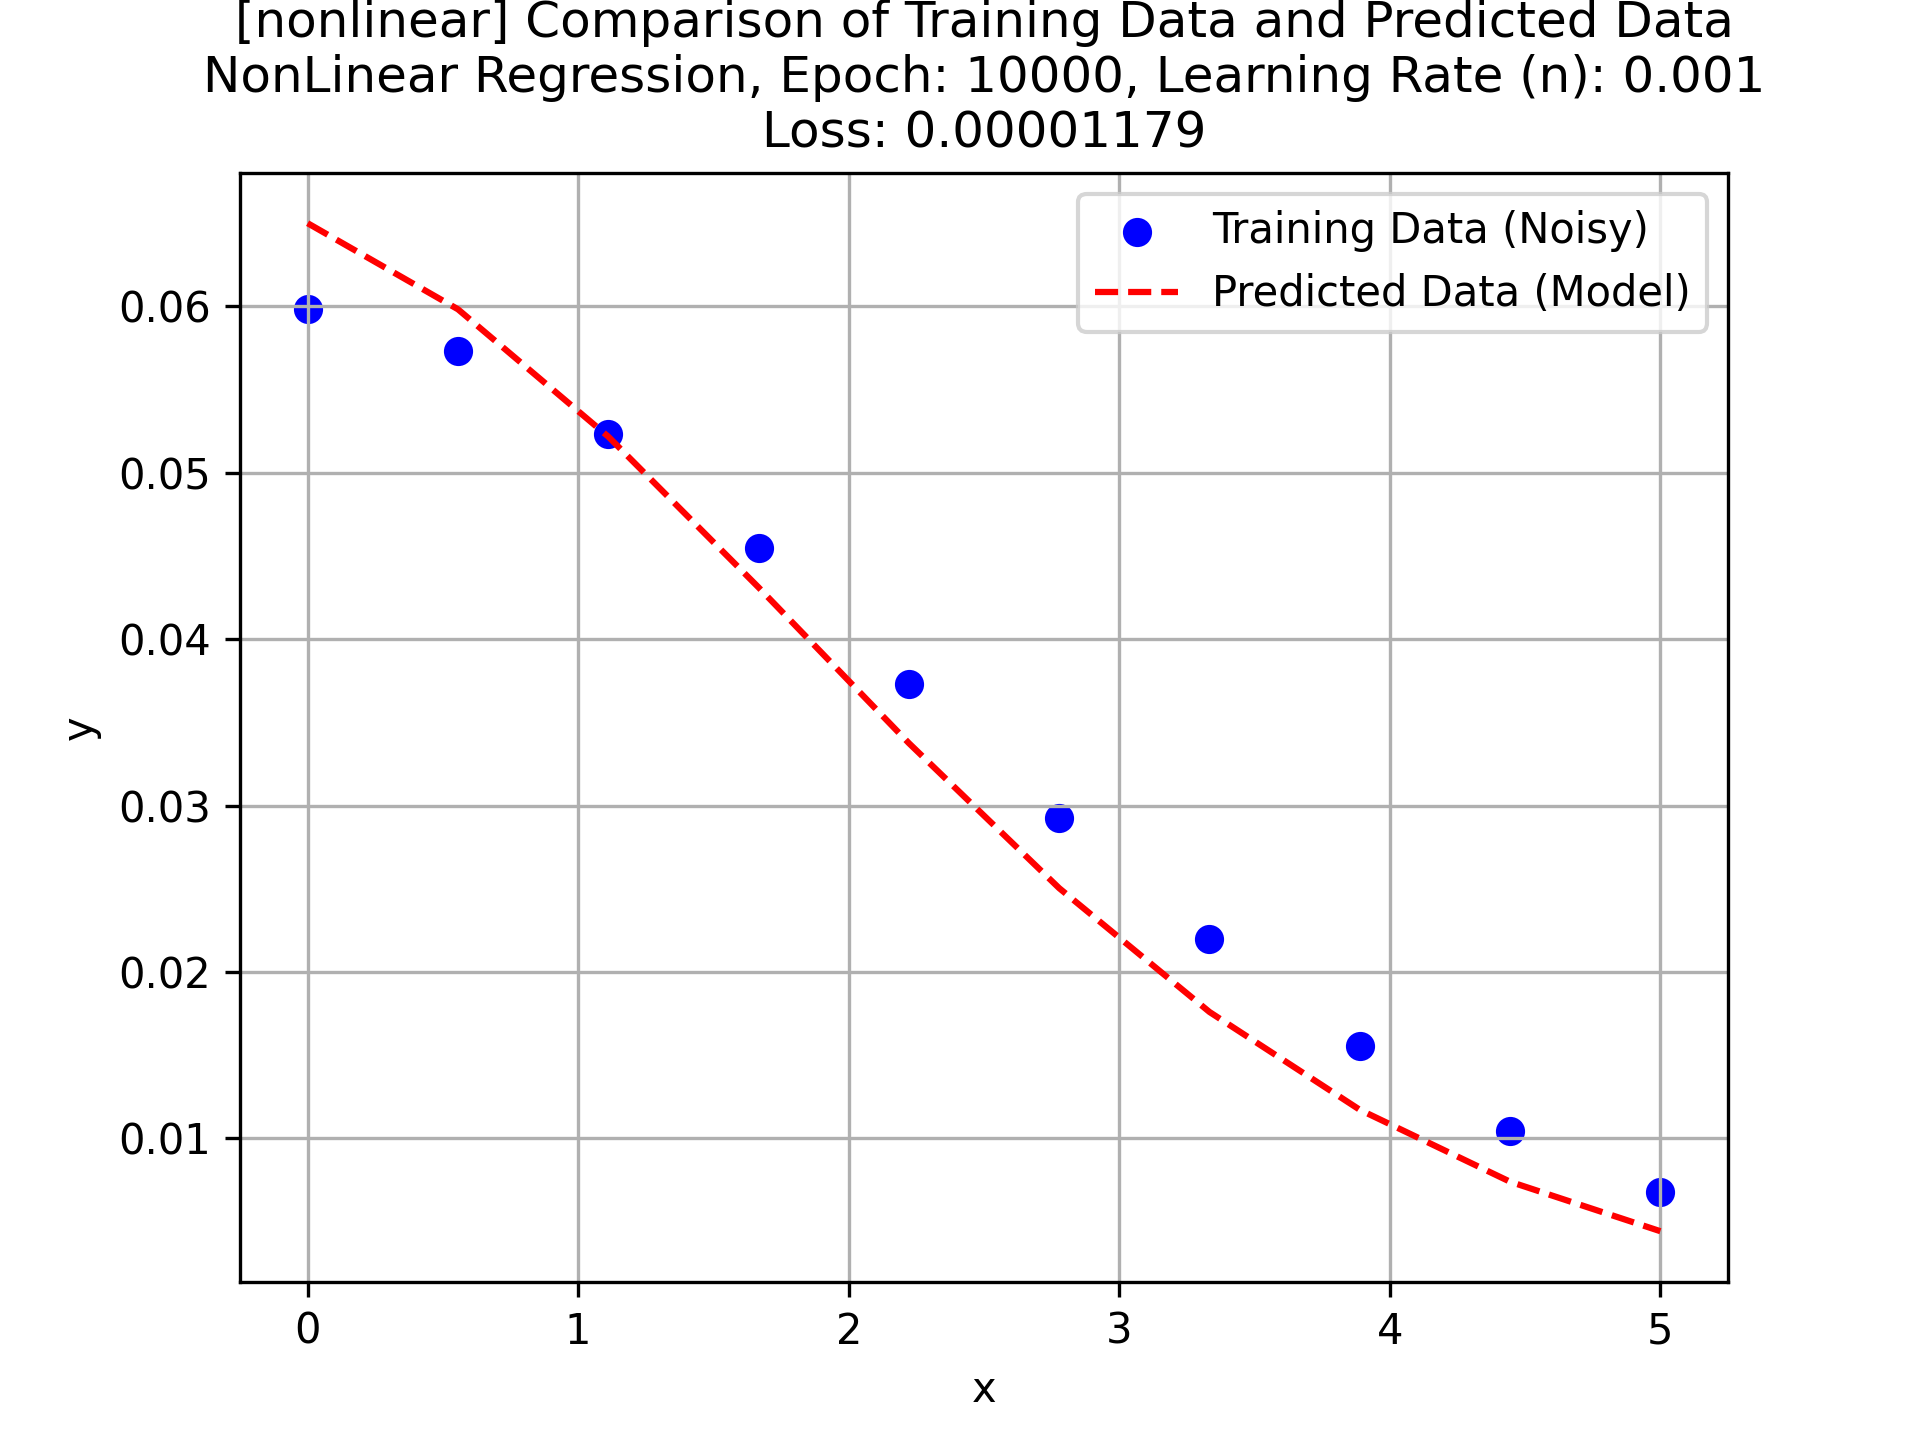
\includegraphics[width=0.8\linewidth]{../Figures/nonlinear_regression_e_10000_n_0.001.png}
   \caption{Nonlinear predicted values $y_{pred}$ versus actual data $y$ with original values }
   \label{fig:NonLin_a}
\end{figure}



\subsection{Results: 2b}
Experiment with the learning rate and the number of epochs.

Here I manually tried different values of epochs and learning rate ($\eta$) and found the set that minimized loss with ensured convergence

\begin{table}[h]
   \centering
   \caption{NonLinear Fit: Table of hyperparameters}
   \label{tab:nonlin_param}
   \begin{tabular}{|c|c|c|c|c|}
      \hline
      Epoch & Learning Rate ($\eta$) & Loss & Convergence & Figure\\
      \hline
      10000 & 0.001 & 0.00001179 & Yes & \ref{fig:NonLin_a}\\
      \hline
      1000 & 0.001 & 0.00005946 & Yes\ & \ref{fig:NonLin_b_less_e}\\
      \hline
      10000 & 0.01 & 0.00007575 & Yes & \ref{fig:NonLin_b_less_n}\\
      \hline
      50000 & 0.0001 & 0.00000775 & Yes & \ref{fig:NonLin_b_min_loss}\\
      \hline
   \end{tabular}
   
\end{table}


% [h!] makes latex try to place figure exactly there, not floating around
\begin{figure}[h!]
   \centering
   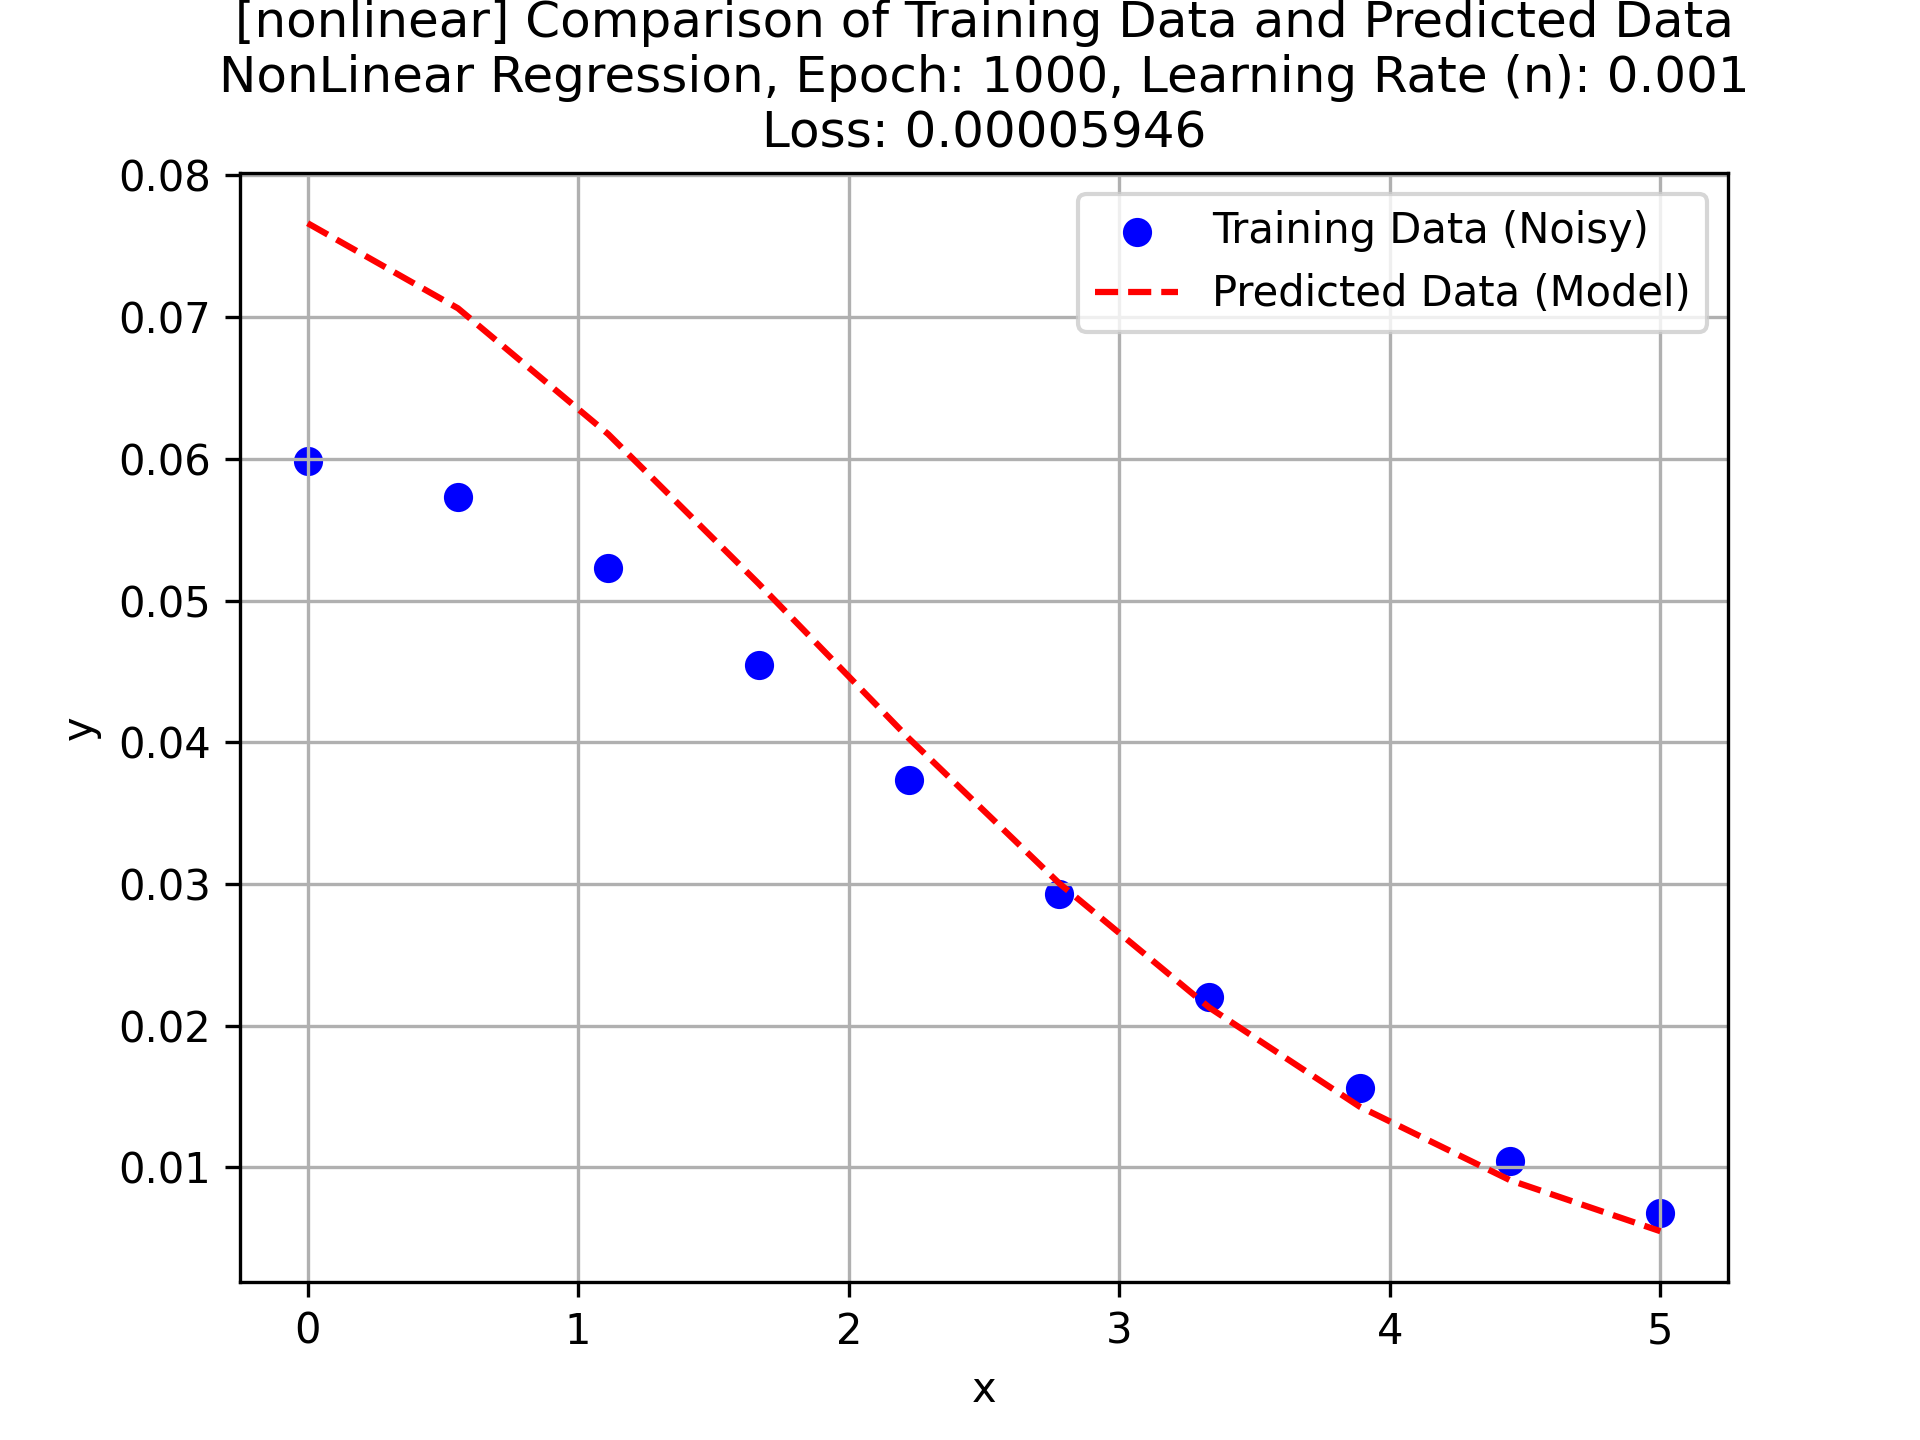
\includegraphics[width=0.8\linewidth]{../Figures/nonlinear_regression_e_1000_n_0.001.png}
   \caption{Predicted values $y_{pred}$ versus actual data $y$ with no convergence}
   \label{fig:NonLin_b_less_e}
\end{figure}

% [h!] makes latex try to place figure exactly there, not floating around
\begin{figure}[h!]
   \centering
   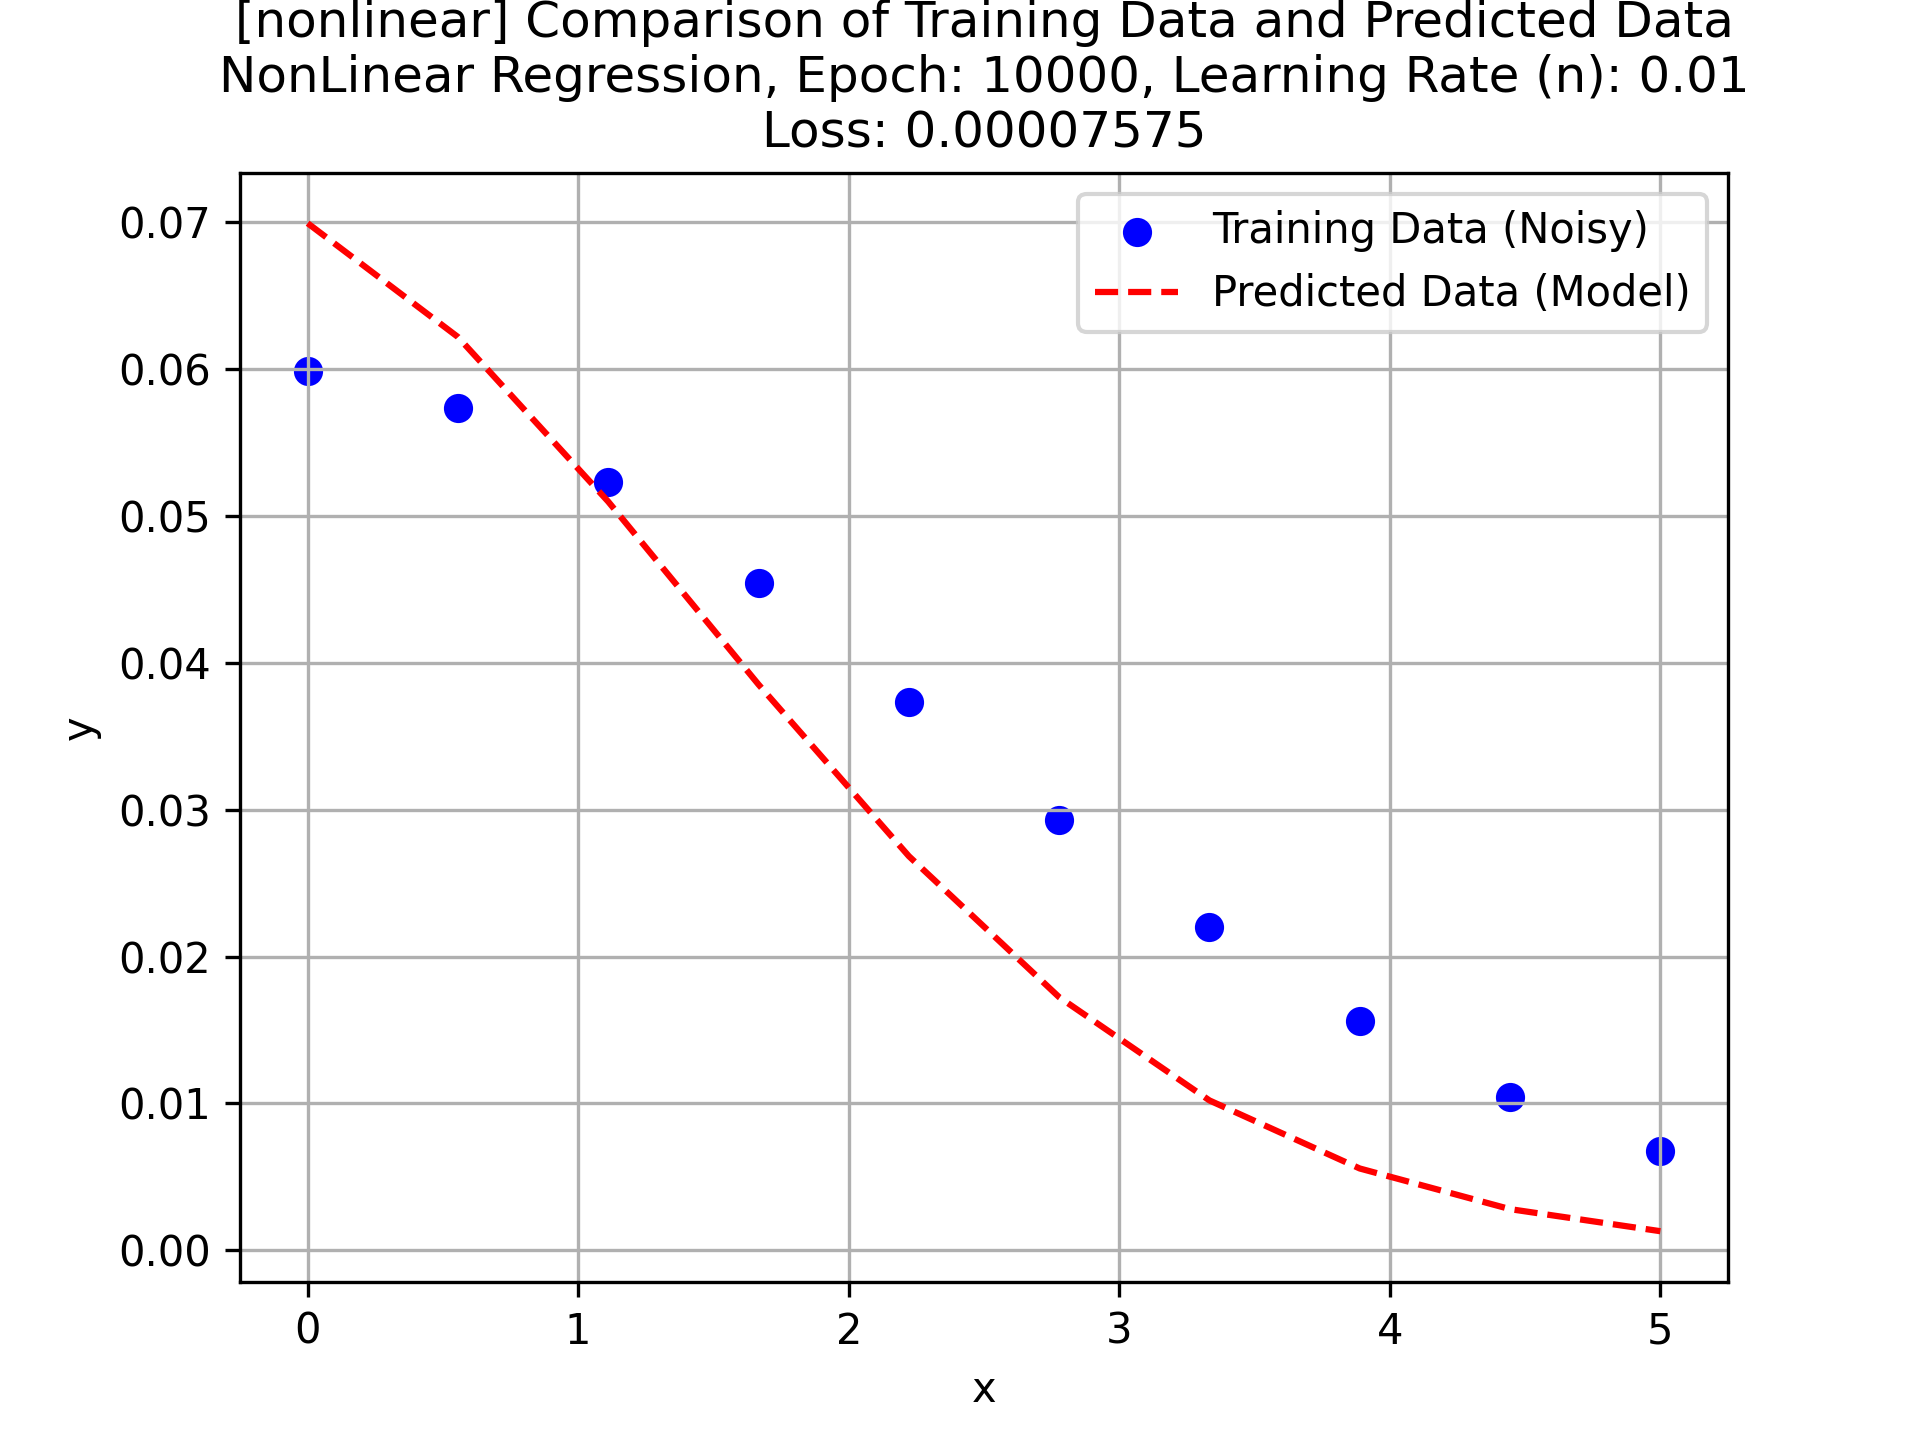
\includegraphics[width=0.8\linewidth]{../Figures/nonlinear_regression_e_10000_n_0.01.png}
   \caption{Predicted values $y_{pred}$ versus actual data $y$ with minimum loss but excess epochs}
   \label{fig:NonLin_b_less_n}
\end{figure}

% [h!] makes latex try to place figure exactly there, not floating around
\begin{figure}[h!]
   \centering
   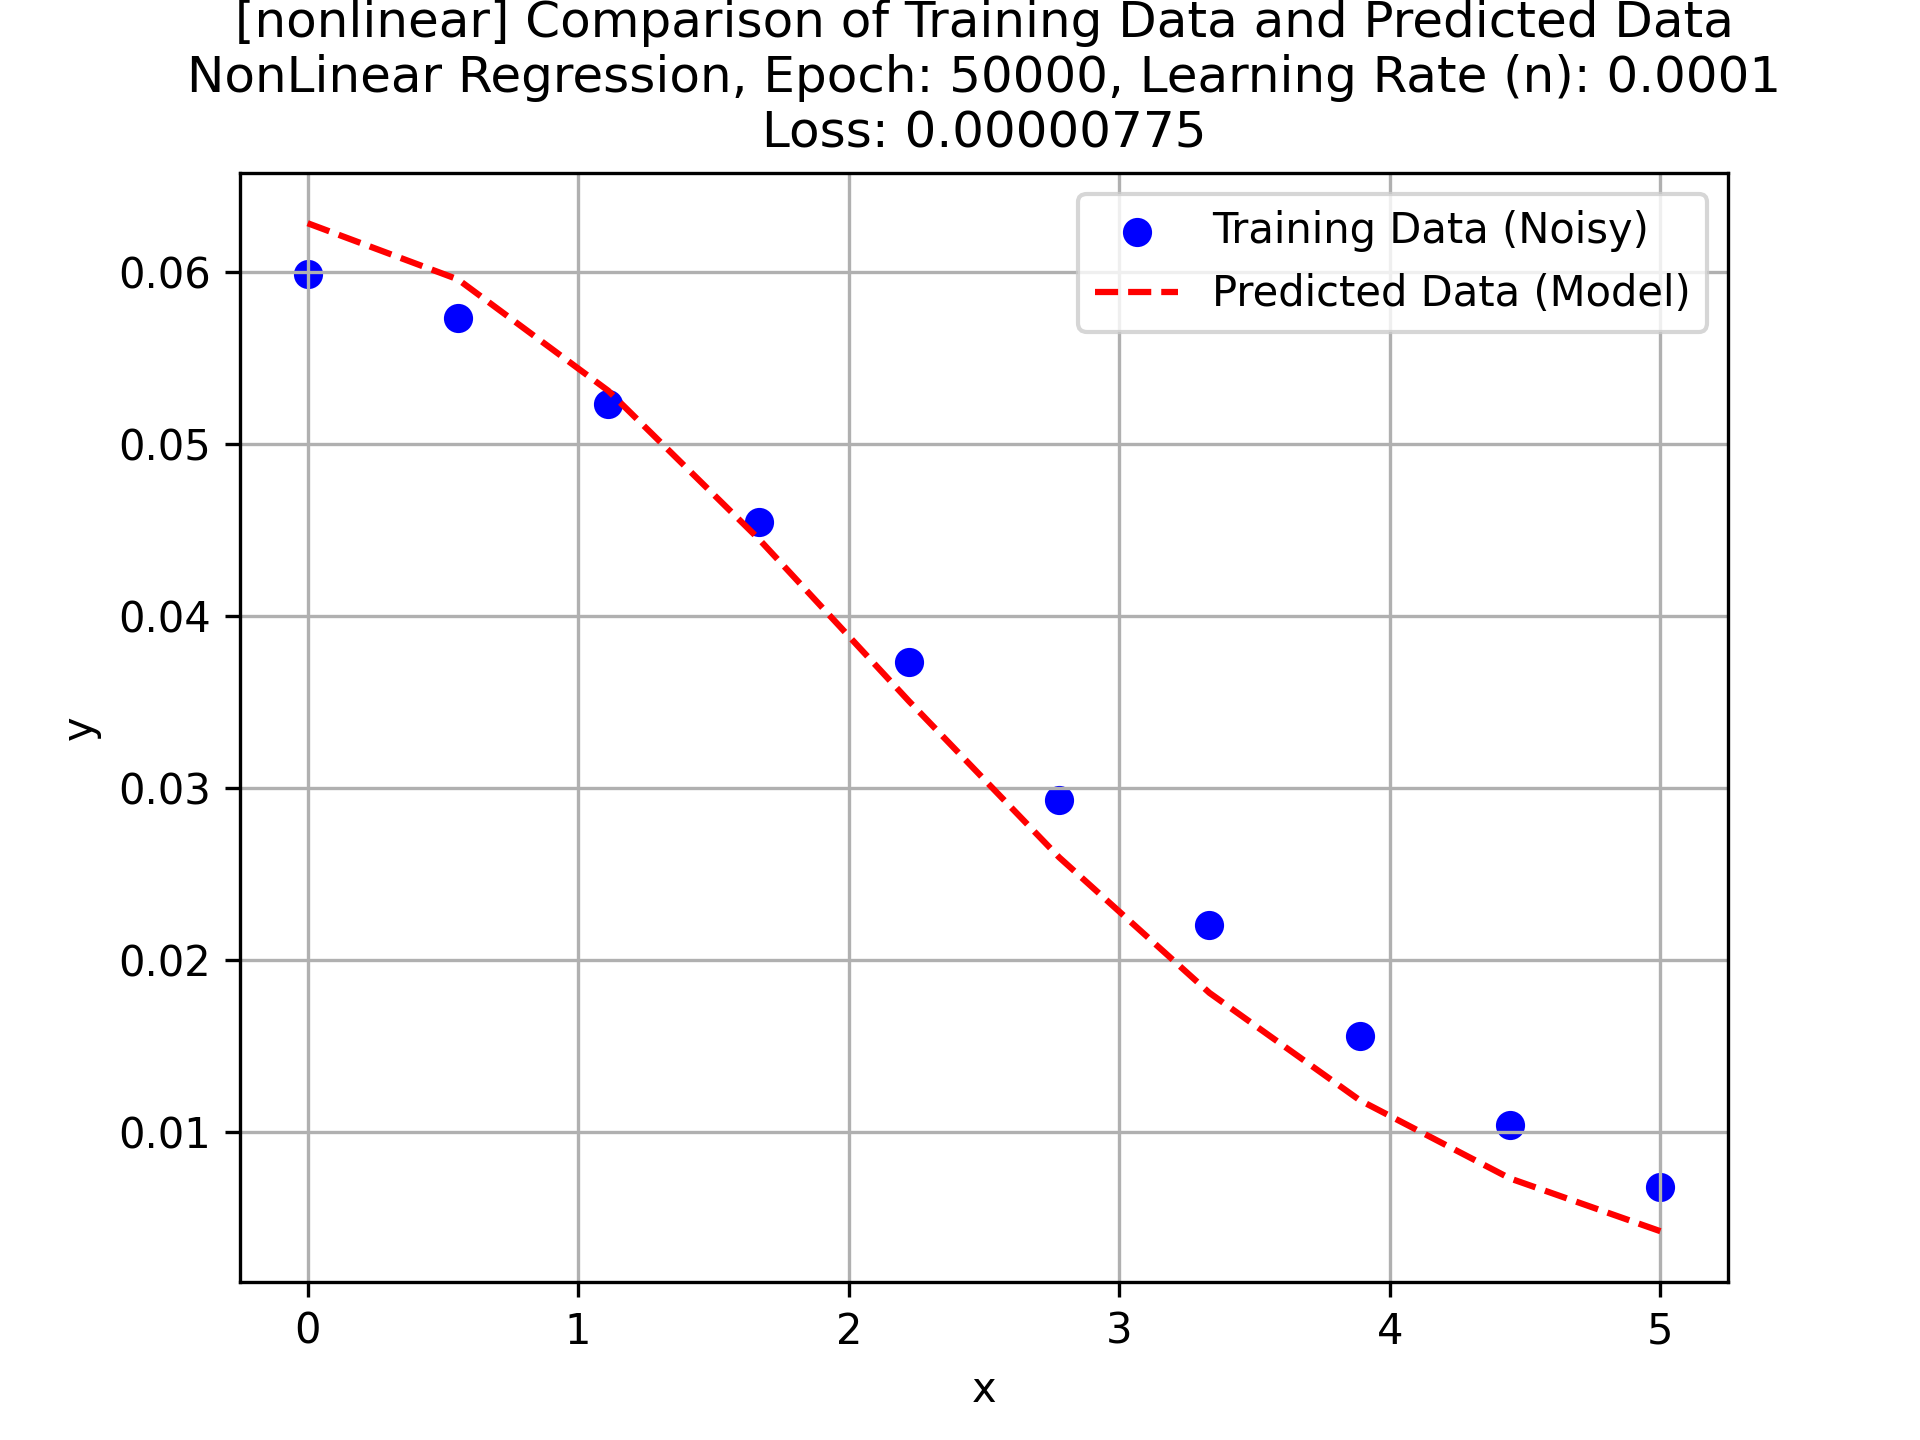
\includegraphics[width=0.8\linewidth]{../Figures/nonlinear_regression_e_50000_n_0.0001.png}
   \caption{Predicted values $y_{pred}$ versus actual data $y$ with minimum loss and optimized epochs}
   \label{fig:NonLin_b_min_loss}
\end{figure}

Changing the learning rate effects the number of epochs required for convergence. 
A smaller learning rate requires more epochs before convergence.
Furthermore, a larger learning rate also affects the precision of the fit, meaning that a minimum loss might not be found because of the larger "steps" from the learning rate. 

Changing the number of epochs affects the final loss, assuming loss is not yet minimized. 
This means there is a minimum number of epochs required to get the optimum fit, and thereafter, higher numbers of epochs are wasted a computation resource.

Together, this means we want a learning rate that is just large enough to find the minimum loss fit, then we want to minimize the number of epochs within this fit.
This was manually found and presented in Figure. \ref{fig:NonLin_b_min_loss}. 

Importantly, we note the qualitative observation that the initial guess for $n$, $a$, $m$, $b$ also have nontrivial effect on the ability for the system to converge, and also on the minimum loss value.
In the code submitted herein, there is logic to pick feasible initial values first before commencing epoch iteration. 
This was required to mitigate the effects of randomness in initial guesses, and to enforce repeatability in the manual, heuristic search of the best hyperparameters. 


%%%%%%%%%%%%%%%%%%%%%%%%%%%%%%%%%%%
\section*{ACKNOWLEDGMENT}

Material used in this report are taken from the course UCLA MAE 263F, Fall 2024.



%%%%%%%%%%%%%%%%%%%%%%%%%%%%%%%%%%%%%%%%%%%%%%%%%%%%%%%%%%%%%%%%%%%%%%%%%%%%%%%%

\begin{thebibliography}{99}

\bibitem{c1} M. Khalid Jawed, Singmin Lim, Discrete Simulation of Slender Structures, UCLA Fall 2024 MAE 263F

\end{thebibliography}


\end{document}
